\chapter{Infraestructura}\label{cap.infraestructura}
En este capitulo se describirán las tecnologías sobre las que se cimienta este trabajo. Para empezar, se detallará el funcionamiento del framework Electron y Node.js, ya que todo el desarrollo de este trabajo será compatible con él. Se profundizará en los dos middleware utilizados, ICE y ROS, y en el entorno JdeRobot. Para finalizar, se describirá el API para el renderizado de gráficos WebGL, concretamente la biblioteca Three.js, y WebRTC para la conexión con los elementos multimedia.

\section{La plataforma JdeRobot}
JdeRobot \footnote{\url{https://jderobot.org/Main_Page}} es el framework de software libre para el desarrollo de robótica y visión artificial creado por el grupo de robótica de la Universidad Rey Juan Carlos y licenciado bajo GPL v3 \footnote{\url{http://www.gnu.org/licenses/gpl-3.0-standalone.html}}. Su desarrollo principalmente está realizado mediante C, C++ y Python, incorporando desarrollo en JavaScript como el tratado en este trabajo.

JdeRobot está basado en componentes que son interconectados mediante el uso de middlewares como ICE o ROS, facilitando el acceso a los dispositivos hardware. Estos componentes obtienen mediciones  de los sensores u ordenes del motor a través de llamadas a funciones locales. JdeRobot conecta esas llamadas a drivers conectados a sensores (para la recepción de las mediciones) o actuadores (para las ordenes), ya sean reales o simulados. Estas funciones locales forman la API de la capa de abstracción. La plataforma también ofrece una serie de herramientas para facilitar la teleoperación o el tratamiento de las mediciones de los sensores, y bibliotecas.

Para el desarrollo de este proyecto, se usará la versión de JdeRobot 5.6.4

\section{El Middleware ICE}
Se trata de un Framework orientado a objetos que ayuda a crear aplicaciones distribuidas fácilmente. ICE se ocupa de todas las interacciones con las interfaces de programación de bajo nivel de red (inhibe al desarrollador de la tarea de apertura de puertos, conexiones de red o serialización de datos). El objetivo principal de ICE es facilitar su uso y el desarrollo de aplicaciones, de modo que en muy poco tiempo se pueda aprender a utilizarlo.

\begin{figure}[H]
  \begin{center}
    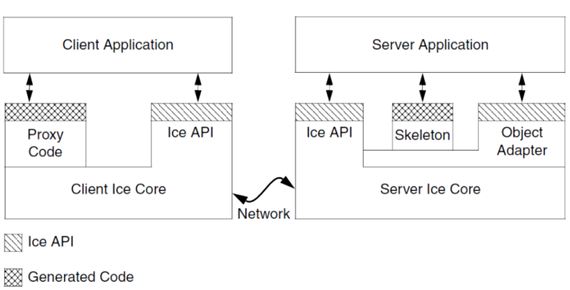
\includegraphics[width=0.8\textwidth]{figures/estructuraice.png}
		\caption{Estructura de Cliente - Servidor con Ice}
		\label{fig.estructurarice}
		\end{center}
\end{figure}

ICE tiene un lenguaje de especificación propio llamado Slice (Specification Language for ICE) que nos permite la abstracción fundamental para separar interfaces de objetos de sus implementaciones. Este lenguaje especifica las interfaces, operaciones y tipos de parámetros utilizados por la aplicación. Cada una de las aplicaciones que queramos que interaccionen entre sí, deben compartir la misma descripción Slice. Esta descripción es independiente del lenguaje en el que está desarrollada nuestro cliente o servidor de modo que sea posible su utilización con clientes y servidores escritos en diferentes lenguajes de programación.

Las interfaces Slice podrían verse como un contrato firmado entre un cliente y un servidor para compartir los mismos tipos, funciones y elementos, dando igual el lenguaje de programación en el que estén escritos, ya que posteriormente se compilan usando el compilador correspondiente al lenguaje de programación correspondiente. Si el cliente y el servidor no compartiesen la misma interface slice, la conexión no podría llevarse a cabo al no conocer las funciones o tipos que maneja cada uno.

Para este trabajo se va a utilizar su versión para JavaScript, sin embargo el soporte para este lenguaje es relativamente reciente, por lo que muchas de las funcionalidades que ofrece para otros lenguajes de programación como C++ o Python, no están disponibles para JavaScript. Sobre todo este hecho es manifiesto en que no hay soporte para la creación de un servidor completo mediante JavaScript, por ello durante este trabajo se ha optado por utilizar ICE únicamente como cliente, con las ventajas e inconvenientes a los que se hará referencia en próximos capítulos.

La versión de ICE que se usará en este trabajo será la 3.6.4

\section{El Middleware ROS}
Se trata de un Framework para el desarrollo de software robótico que ofrece las funcionalidades de un sistema operativo (abstracción del hardware, control de dispositivos de bajo nivel, mantenimiento de paquetes, etc.). ROS ofrece una serie de herramientas, bibliotecas y convenciones para simplificar la tarea de crear complejos y robustos robots. Nace con la idea de fomentar el desarrollo colaborativo, es decir que cualquier persona que realice un desarrollo puede subir a los repositorios que ofrece ROS para ello, de modo que otra persona pueda utilizarlo para usarlo en su proyecto.

El elemento fundamental del funcionamiento de ROS es el nodo. Un nodo es un proceso que realiza cálculos y se comunican entre sí mediante un sistema de publicación - subscripción para conexiones asíncronas y anónimas, o servicios para las conexiones síncronas. Los nodos operan en una escala de bajo nivel, es decir cada nodo se ocupa de un parte del sistema de control de robot, por ejemplo un nodo se ocupa de los motores, otro nodo se ocupa de realizar la localización, etc. Este elemento proporciona mayor tolerancia a los fallos al ser bloques separados y aislados, y se reduce la complejidad del código.

En el sistema de comunicación asíncrona, un nodo actúa como publicador que transmite un mensaje con una etiqueta llamada topic por el canal para que sea recibido por cualquier otro nodo que se subscriba a esta etiqueta o topic. El mensaje enviado es una estructura de datos simple, que comprende campos tipados. ROS ofrece una serie de formatos de mensajes estándar que cubren la mayoría de necesidades de uso común (mensajes para sensores, cámaras, movimiento, láseres, nubes de puntos, etc).

\begin{figure}[H]
  \begin{center}
    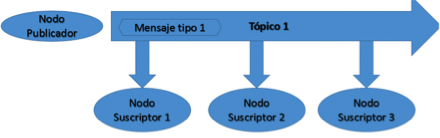
\includegraphics[width=0.8\textwidth]{figures/publicadorsubscriptor.png}
		\caption{Estructura del sistema de comunicación Publicador - Subscriptor}
		\label{fig.publicadorsubscriptor}
		\end{center}
\end{figure}

El sistema de comunicación síncrona, es el típico sistema cliente-servidor a través del cual un nodo ROS es el prestador del servicio que permanece en escucha continua y el resto de nodos le envían mensajes de solicitud. Cada servicio está definido por el tipo de servicio que define la cantidad y tipo de datos que necesita el servicio tanto para recibir como petición, como para enviar como respuesta.

\begin{figure}[H]
  \begin{center}
    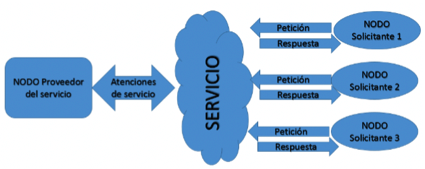
\includegraphics[width=0.8\textwidth]{figures/serviciosros.png}
		\caption{Estructura del sistema de comunicación por Servicios ROS}
		\label{fig.serviciosros}
		\end{center}
\end{figure}

Un elemento que es muy útil para este proyecto es que ROS nos proporciona total compatibilidad con Gazebo mediante un conjunto de paquetes llamados \textit{gazebo\_ros\_pkgs} \footnote{\url{http://wiki.ros.org/gazebo_ros_pkgs}}. En ROS, los paquetes son aquellos donde se incluye todo el código fuente, las librerías usadas y cualquier otro recurso necesario para que funcione el nodo.

La versión de ROS que se utilizará para el desarrollo de este trabajo es ROS Kinetic.

\section{Robot Web Tools}
Comunidad nacida a partir de la de ROS, nos permite conectar aplicaciones web a elementos robóticos gracias a un protocolo llamado Rosbridge. Este protocolo es una especificación de JSON para interactuar con ROS y una capa de transporte para que los clientes se comuniquen mediante WebSockets. Por otro lado, han creado una serie de bibliotecas livianas y fáciles de utilizar de JavaScript que proporcionan una  abstracción de la funcionalidad principal de ROS. Estas bibliotecas son roslibjs, ros2djs y ros3djs, sin embargo en este trabajo solo se utilizará roslibjs.

La biblioteca roslibjs es la encarga de ofrecernos las funcionalidades necesarias para conectarnos, enviar o recibir mensajes ya sea mediante publicación y subscripción, o servicios. La conexión se realiza a un servidor intermedio (servidor Rosbridge), el cual se encarga de gestionar las conexiones, los topic publicados o los servicios activos en cada momento, de modo que cuando te subscribas o realices la petición de un servicio, este servidor se encargue de encaminar la petición mediante WebSockets.

Dado que para este trabajo se va a utilizar JavaScript como lenguaje, se utilizará, en todas las partes relacionadas con ROS, las bibliotecas, servidores y protocolo indicado en esta sección.

\begin{figure}[H]
  \begin{center}
    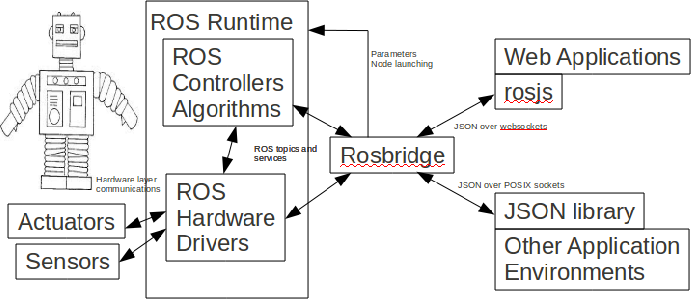
\includegraphics[width=0.8\textwidth]{figures/estructurarosbridge.png}
		\caption{Estructura de una aplicación con Rosbridge}
		\label{fig.estructurarosbridge}
		\end{center}
\end{figure}

\section{Node.js}
Node.js \footnote{\url{https://nodejs.org/es/}} es un entorno multiplataforma del lado del servidor. Concebido con la intención de facilitar la creación de programas de red escalables como puede ser un servidor web, nos permite ejecutar código JavaScript fuera de un navegador y aprovechar las ventajas que nos proporciona su programación orientada a eventos. Su ejecución se lleva a cabo en un único hilo, usando entradas y salidas asíncronas que pueden ejecutarse de manera concurrente, provocando que cada una de ellas necesite de un callback para manejar los eventos. 

Node.js proporciona una serie de módulos básicos que permiten realizar funciones esenciales como puede ser la programación en red asíncrona, el manejo de archivos del sistema, etc. Sin embargo, al ser de código abierto, existe una gran comunidad de desarrolladores que crean nuevos módulos para que cualquiera pueda utilizarlos. Estos módulos son fácilmente compartidos gracias al manejador de paquetes npm \footnote{\url{https://www.npmjs.com/}}, permitiéndonos compilar, instalar y manejar las dependencias de cualquier módulo de terceros que deseemos usar en nuestro proyecto.
 
Por lo general, un proyecto Node.js contendrá al menos dos elementos, un archivo .js que contendrá la lógica del programa escrita en JavaScript y un segundo archivo llamado Package.json que definirá nuestro programa. Este segundo archivo es donde se indican las dependencias que usará nuestro programa y nos facilitará su instalación conjunta usando el comando npm install, así como se referenciará al fichero .js indicado anteriormente.

La versión de Node.js utilizada será la 8.9.1 y la versión del manejador de paquetes npm será la 6.4.0.

\section{WebGL y Three.js}
WebGL \footnote{\url{https://get.webgl.org/}}  es un API multiplataforma utilizada para crear gráficos 3D utilizando tecnologías web, está basado en OpenGL y utiliza parte de su API. WebGL se ejecuta dentro del elemento HTML Canvas, o que proporciona una completa integración con la interfaz DOM. Ofrece ventajas como la compatibilidad con distintos navegadores y plataformas, no es necesario compilar para su ejecución o la interacción con otros elementos del HTML. Sin embargo, debido a que se trata de un API de bajo nivel es complejo de utilizar.

Three.js \footnote{\url{https://threejs.org/}} nace como remedio a la complejidad de usar WebGL. Se trata de una biblioteca desarrollada en JavaScript que permite crear y mostrar gráficos 3D en un navegador web usando una API de alto nivel, proporcionados funciones y objetos para facilitar la creación, interacción y visualización de entornos con gráficos 3D. Utilizando secuencias de código tan simples como \textsl{object = new THREE.Mesh( new THREE.SphereBufferGeometry(75, 20, 10), new THREE.MeshBasicMaterial({color:0xFF0000}))}, nos permite crear una esfera siendo la primera parte donde se define la geometría y la segunda donde se establece el material (puede ser desde un color básico como en este caso, hasta una textura obtenida desde una imagen)

\begin{figure}[H]
  \begin{center}
    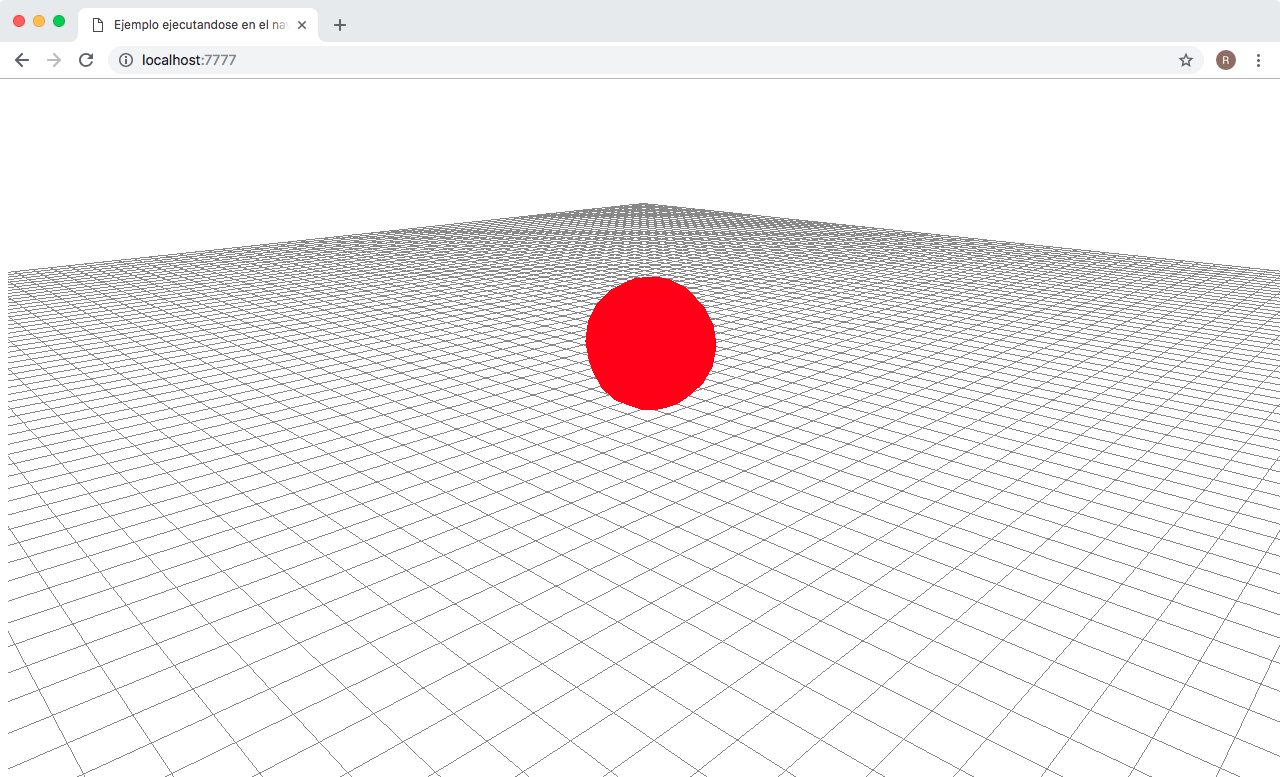
\includegraphics[width=0.8\textwidth]{figures/esferathreejs.png}
		\caption{Esfera creada con la biblioteca Three.js y mostrada en un navegador}
		\label{fig.esferathreejs}
		\end{center}
\end{figure}

\section{WebRTC}
WebRTC \footnote{\url{https://webrtc.org/}}  una tecnología que permite a una aplicación web capturar y transmitir audio y video, así como intercambiar datos con otros navegadores sin necesidad de intermediarios. Este intercambio se realiza de igual a igual (peer-to-peer) sin necesidad de instalaciones o software adicionales. WebRTC proporciona varias API y protocolos interrelacionados para dar a los navegadores y aplicaciones móviles la capacidad de intercambiar elementos multimedia en tiempo real (Real Time Communications). Esta tecnología esta soportada en los principales navegadores y tiene el soporte de Google.

En este proyecto, usaremos WebRTC para la adquisición de del video obtenido a través de una cámara web. Para lograr este objetivo, se utilizará el API de WebRTC Media Stream, que nos proporcionará la descripción de los flujos de datos de audio y video, los métodos para trabajar con ellos, la conexión con los dispositivos para adquirirlos, las limitaciones asociadas a cada tipo de datos o los eventos asociados al proceso.

\section{El framework Electron}
Electron \footnote{\url{https://electronjs.org/docs}}  es un framework de código abierto desarrollado por GitHub. Comenzó su desarrollo en 2013, en el mismo grupo de trabajo del editor Atom \footnote{\url{https://atom.io/}}. Concebido con la ides de permitir la creación de aplicaciones de escritorio multiplataforma con tecnologías web. Electron es la combinación de NodeJS y Chromium \footnote{\url{https://www.chromium.org/Home}} en una misma ejecución.

La arquitectura de una aplicación que utiliza Electron esta formada por dos procesos: Principal y Renderizador. 

El proceso principal es el encargado de generar la interfaz de usuario mediante la creación de páginas web y las administra de modo que es posible mostrar más de una página web al mismo tiempo. Esta labor se realiza mediante la instancia al objeto BrowserWindow de Electron, ejecutándose una página web cada vez que se instancia. Cuando se destruye una de estas instancias, se está cerrando esa página web. Cada aplicación con Electron debe constar de un único proceso principal, y corresponderá al script main del archivo package.json.

El proceso renderizador es cada instanacia al objeto BrowserWindow y la ejecucuion de la página web correspondiente. Una aplicación con Electron puede tener multitud de procesos renderizadores, siendo cada uno independiente del resto. Cada proceso solos se preocupa de la página web que se esta ejecutando en él.

Electron es totalmente compatible con NodeJS tanto en el proceso principal como en el renderizador, por lo que todas las herramientas disponibles para Node.js, también lo están para Electron. Así mismo, es posible utilizar módulos Node.js alojados en el repositorio de paquetes npm mencionado anteriormente. Este nos aporta un gran número de ventajas como una mayor seguridad al cargar contenido remoto, tener siempre actualizadas las aplicaciones o tener un gran número de bibliotecas disponibles.

Todas las aplicaciones que se desarrollarán en este trabajo podrán ser ejecutadas utilizando Electron, lo que nos permite utilizarlas en cualquier plataforma o, incluso, empaquetarlas usando npm o mediante un archivo Asar \footnote{\url{https://github.com/electron/asar}}.

\subsection{Adaptar una aplicación web para ser usada con Electron}

Una aplicación que utiliza Electron estará formada por un archivo HTML, un fichero main.js que definirá la ventana donde se mostrará el fichero HTML y se creará la misma, y, al igual que se indica en la sección de Node.js, el archivo package.json que definirá la aplicación en Electron (nombre, versión, descripción, etc.), se indicaran las dependencias a módulos externos y el fichero main.js para que creé la aplicación. Una vez que contamos con al menos estos tres elementos, podemos instalar las dependencias mediante npm install (igual que para Node.js) y ejecutar la aplicación mediante npm start o npm test (dependerá de como hayamos definido package.json).

\subsubsection{package.json}
El cometido de este archivo definirá las dependencias de paquetes de terceros que tendrá la aplicación web, definir las características de la aplicación (nombre, versión, autor, etc.) y, lo que es más importante, de que manera se lanzara la aplicación y el archivo que se debe ejecutar al lanzarla. A continuación se muestra lo que podría ser un ejemplo de un package.json:
\begin{lstlisting}[frame=single]
{
  "name": "Ejemplo",
  "version": "0.1.0",
  "main": "main.js",
  "scripts": {
    "start": "electron ."
  },
  "dependencies": {
      "electron": "^1.8.4",
  }
}
\end{lstlisting}

Como se puede apreciar, la versión de Electron que se utilizará será la 1.8.4.

\subsubsection{main.js}
El archivo "main.js" indicado anteriormente, contendrá muy pocas líneas de código al tratarse de un elemento totalmente externo a la aplicación y no tener ningún papel en su funcionamiento, únicamente es necesario para ejecutar la aplicación utilizando Electron. A continuación se muestra el código de este archivo:

\begin{lstlisting}[frame=single]
const app = require('electron')
const path = require('path')
const url = require('url')

let win;

function createWindow () {
  win = new BrowserWindow({width: 1800, height: 1000})
  win.loadURL(url.format({
    pathname: path.join(__dirname, 'camserver.html'),
    protocol: 'file:',
  }))
  
app.on('ready', createWindow)

\end{lstlisting}

Lo primero que se realiza es definir los módulos que se requieren para que funcione correctamente y que se utilizaran en el resto del código. Posteriormente, se define el tamaño de la ventana, en este caso la ventana será de 1800 pixeles de ancho y 1000 de alto. Mediante win.loadURL se simula el funcionamiento de un navegador y como gestionan las diferentes URLs, este método se le pasará como parámetros el archivo HTML principal de la aplicación web, el protocolo que este caso es "file:", al estar queriendo mostrar directamente de un archivo HTML (si quisiéramos mostrar mediante Electron el contenido de una página web ya existente, protocol tomaría el valor "http:"). Finalmente, la última línea de código llamará a la función que crea la ventana y muestra el HTML en el momento que Electron haya terminado de inicializarse y está preparado para la creación de la ventana.


En la figura 3.6 se muestra el mismo HTML ejecutado con Node.js y con Electron. Como se puede apreciar, el resultado es el mismo.

\begin{figure}[H]
  \begin{center}
    \subfigure[Node.js]{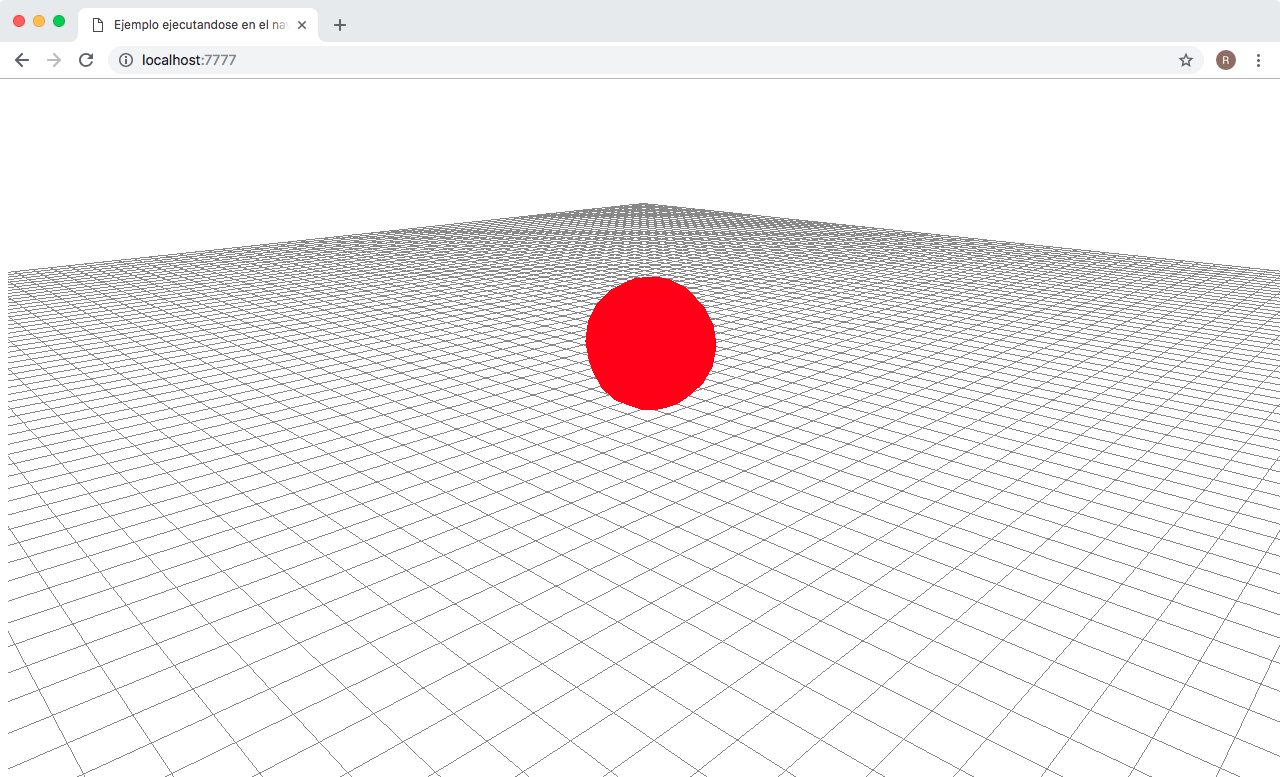
\includegraphics[width=0.4\textwidth]{figures/esferathreejs.png}}
    \subfigure[Electron]{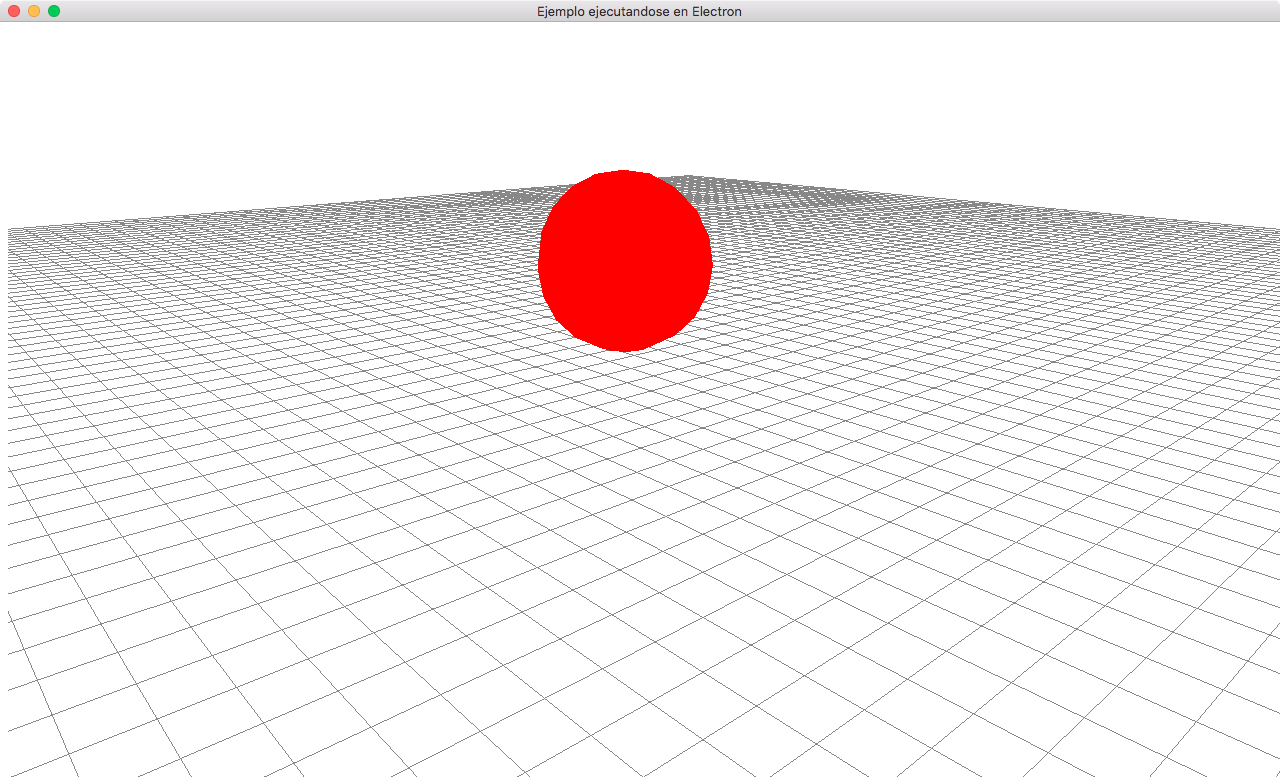
\includegraphics[width=0.4\textwidth]{figures/ejemploelectron.png}}
    \caption{Ejemplo de la esfera anterior ejecutado con Node.js y con Electron}
     \label{fig.ejemplohtmlcomm}
     \end{center}
\end{figure}






